
%(BEGIN_QUESTION)
% Copyright 2008, Tony R. Kuphaldt, released under the Creative Commons Attribution License (v 1.0)
% This means you may do almost anything with this work of mine, so long as you give me proper credit

Sketch the necessary wiring to make this pressure switch control two lamps in the following manner:

\begin{itemize}
\item{} High process pressure: red lamp on and green lamp off
\item{} Low process pressure: Green lamp on and red lamp off
\end{itemize}

$$\includegraphics[width=15.5cm]{i03250x01.eps}$$

\vfil 

Hint: remember that the ``normal'' status of a switch is defined as the status of {\it minimum stimulus}: when the switch is exposed to the lowest possible degree of process stimulation (in this particular case, to the lowest possible pressure).

\underbar{file i03250}
\eject
%(END_QUESTION)





%(BEGIN_ANSWER)

This is a graded question -- no answers or hints given!
 
%(END_ANSWER)





%(BEGIN_NOTES)

This is just one possible solution:

$$\includegraphics[width=15.5cm]{i03250x02.eps}$$

If ``normal'' for a switch contact means ``minimum stimulus,'' then we know at low pressure this switch's NO contact will be open and its NC contact will be closed.  The opposite states occur at pressures above the switch's trip point.  Thus we need to wire the green lamp to receive power through the NC switch contact, and for the red light to receive power through the NO switch contact.

%INDEX% Pictorial circuit review (process switch circuit)

%(END_NOTES)


